%% 第三届“空天杯”全国创新创意大赛初赛论文Latex模版
%% 作者:Seafood
%% 联系方式:qq993146483
\documentclass{sky}
\title{论文题目}
\author{作者1 \quad 作者2 \vspace{10pt}\\ \zihao{-5}{(单位)\vspace{10pt}}\\ {\kaishu \zihao{5}负责人:XX, 联系方式:xxxxxx,邮箱:xxxxxx}}
\date{2021.5}
\begin{document}
    \begin{titlepage}
        \maketitle

    \end{titlepage}
    

    %%摘要
    \begin{abstract}
        \onehalfspacing
    %\noindent
    {\heiti{摘要:}}摘要

    %\noindent
    {\heiti{关键词:}}关键词1,关键词2
    \end{abstract}
    
    \newpage
    \tableofcontents
    \newpage
    \section{概述}
    概述\cite{artwritingscientific-Geer-2000}。
    \subsection{研究背景和需求分析}
    \subsubsection{研究背景}
    \begin{figure}[htbp]
        \centering
        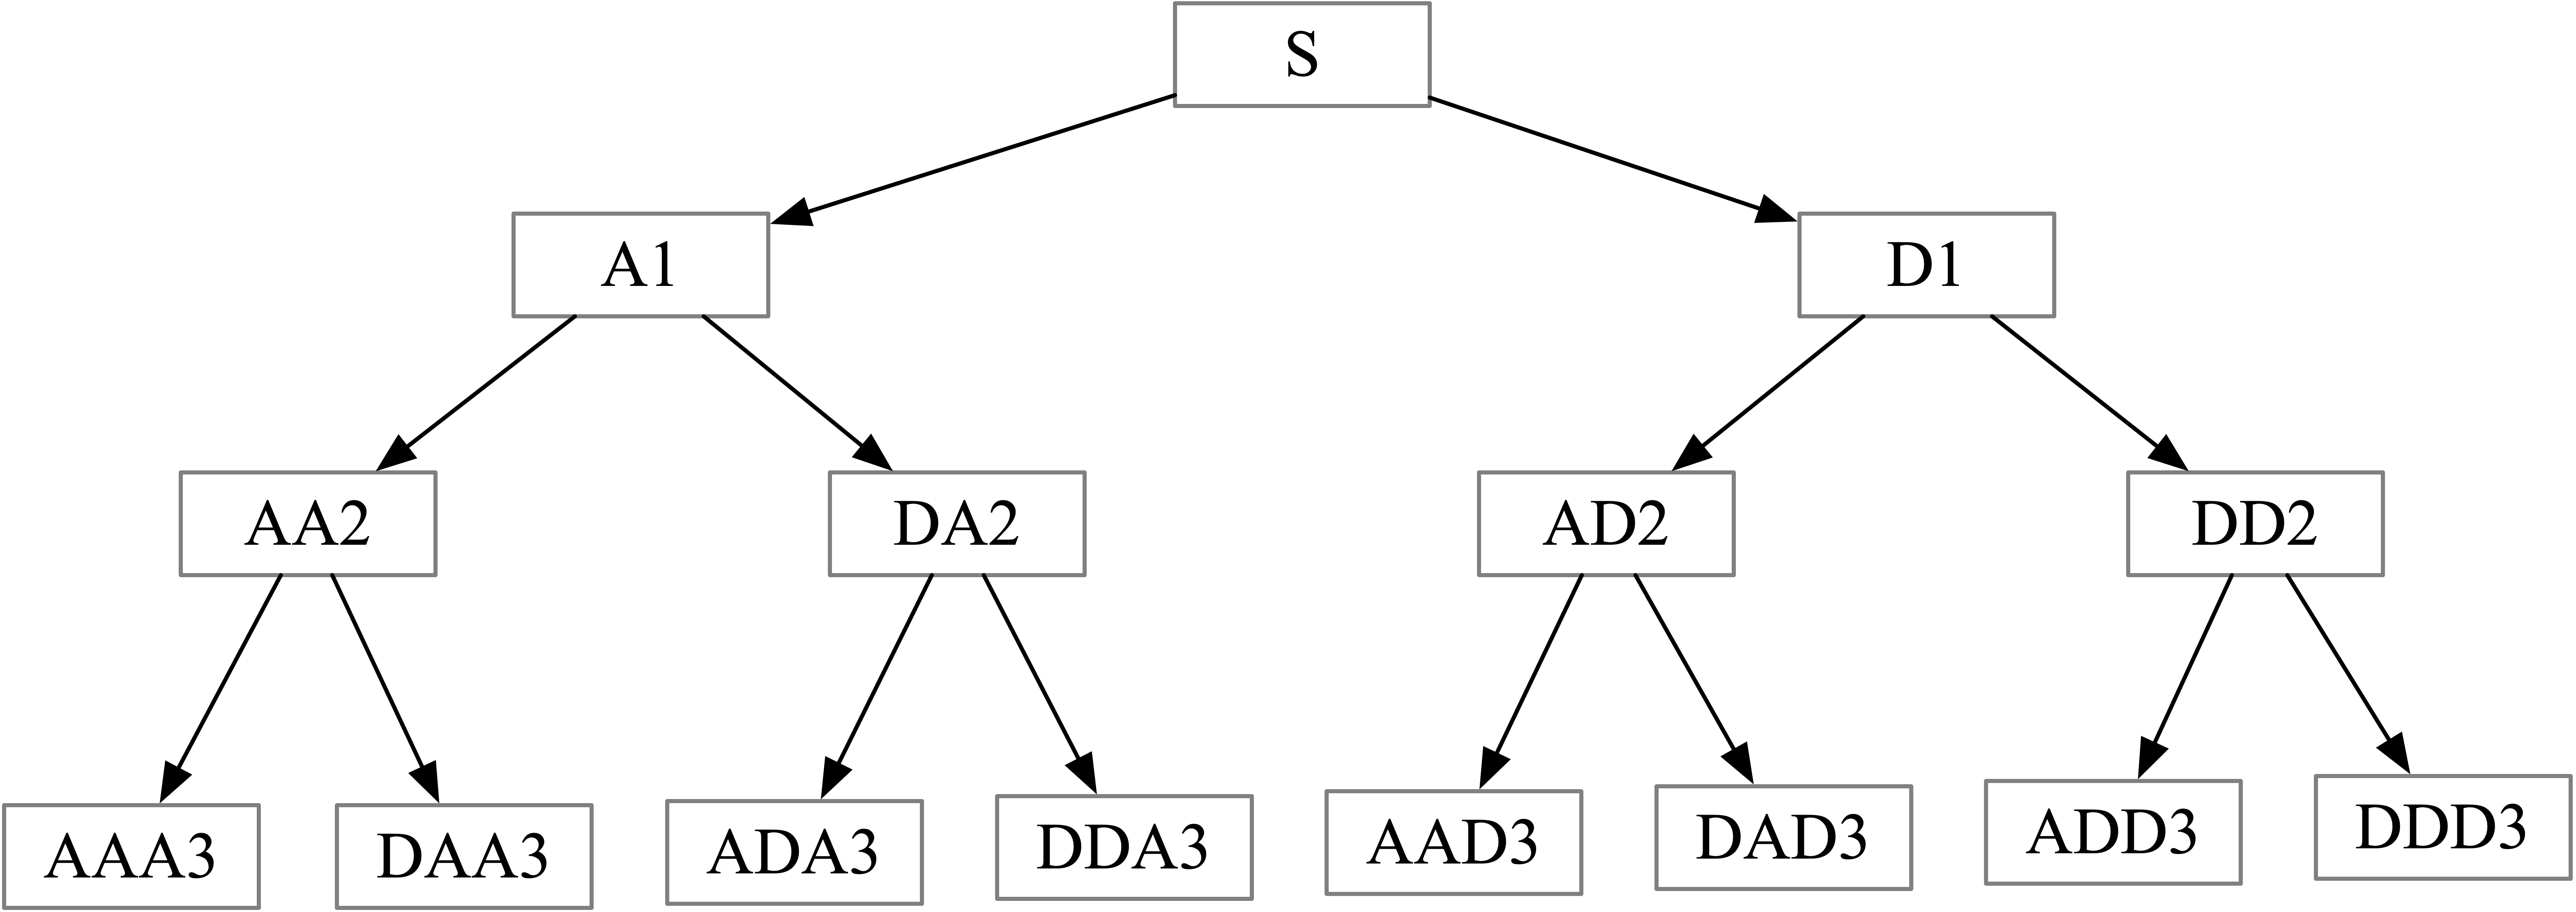
\includegraphics[width=0.7\textwidth,scale=1.0]{pictures/waveletpacket.png}
        \caption{空间态势感知中的层次化数据融合技术模型}
        \label{networkdiagram}
    \end{figure}
    \subsubsection{需求分析}
    \section{方案描述}
    \section{可行性分析}
    \section{创新性分析}
    \section{应用前景分析}
    \section{总结和展望}

    \begin{myfigureandtable}
        \listoffigures

        \listoftables
    \end{myfigureandtable}

    \begin{myreference}
        \bibliographystyle{plain}
        \bibliography{reference}
    \end{myreference}
    
\end{document}